\documentclass[a4paper,12pt]{article}
\usepackage[
    a4paper, bindingoffset=0.2in, left=10mm, right=10mm, 
    top=30mm, bottom=27mm, footskip=5.5mm, headheight=15mm      % tuve que cambiar el bottom porque queda no imprimible por mi impresora
]{geometry}
\usepackage{amsmath, accents, graphicx, caption, siunitx, float, fancyhdr, lastpage}
\usepackage[bookmarks]{hyperref}
\newcommand*\rfrac[2]{{}^{#1}\!/_{#2}}
\newcommand{\im}[1]{j\; #1} 
\newcommand{\parallelTwo}[2]{\left.#1\,\middle/\!\middle/\,#2\right.}

\newcommand{\mR}[1]{\SI{#1}{\kilo\ohm}}
\newcommand{\mI}[1]{\SI{#1}{\milli\ampere}}
\newcommand{\mIu}[1]{\SI{#1}{\micro\ampere}}
\newcommand{\mV}[1]{\SI{#1}{\volt}}

% ------------ Header and Footer --------------------
\pagestyle{fancy}
\lhead{
\includegraphics[height=15mm]{./imagenes/Logo_UTN.png}}
\chead{
    \textsc{Electrónica Aplicada I} \\
    \footnotesize {Departamento de Electrónica} \\
    \footnotesize {Trabajo Práctico de Laboratorio. Período Lectivo 2019}
}
\rhead{}
\lfoot{ 
    \small{\textit{Grupo:}} \\
    \footnotesize{\textsc{Sukanec, Sanahuja, Caprula, Viña, Ortolan}}
}
\cfoot{}
\renewcommand{\footrulewidth}{0.4pt}% default is 0pt
\rfoot{\small{ Pag \thepage \; de \pageref*{LastPage} }}


% ---------------------- Inicio Documento -------------------
\begin{document}
%%%%%%%%%%%%%%%%%%%%%%%%%%%%%%%%%%%%%%%%%
% Academic Title Page
% LaTeX Template
% Version 2.0 (17/7/17)
%
% This template was downloaded from:
% http://www.LaTeXTemplates.com
%
% Original author:
% WikiBooks (LaTeX - Title Creation) with modifications by:
% Vel (vel@latextemplates.com)
%
% License:
% CC BY-NC-SA 3.0 (http://creativecommons.org/licenses/by-nc-sa/3.0/)
% 
% Instructions for using this template:
% This title page is capable of being compiled as is. This is not useful for 
% including it in another document. To do this, you have two options: 
%
% 1) Copy/paste everything between \begin{document} and \end{document} 
% starting at \begin{titlepage} and paste this into another LaTeX file where you 
% want your title page.
% OR
% 2) Remove everything outside the \begin{titlepage} and \end{titlepage}, rename
% this file and move it to the same directory as the LaTeX file you wish to add it to. 
% Then add \input{./<new filename>.tex} to your LaTeX file where you want your
% title page.
%
%%%%%%%%%%%%%%%%%%%%%%%%%%%%%%%%%%%%%%%%%

%----------------------------------------------------------------------------------------
%	PACKAGES AND OTHER DOCUMENT CONFIGURATIONS
%----------------------------------------------------------------------------------------

% \documentclass[11pt]{article}
% \usepackage[utf8]{inputenc} % Required for inputting international characters
% \usepackage[T1]{fontenc} % Output font encoding for international characters
% \usepackage{mathpazo, graphicx} % Palatino font
% \begin{document}

%-------------------------------- TITLE PAGE -----------------------------------	
\begin{titlepage} % Suppresses displaying the page number on the title page and the subsequent page counts as page 1
	\newcommand{\HRule}{\rule{\linewidth}{0.5mm}} % Defines a new command for horizontal lines, change thickness here
	\center % Centre everything on the page
	
	%------------------- Headings -----------------------------
	\textsc{\LARGE Universidad Tecnológica \\[5pt] de Buenos Aires}\\[1.5cm] % Main heading such as the name of your university/college
	\textsc{\Large Electrónica Aplicada I}\\[0.5cm] % Major heading such as course name
	\textsc{\large Trabajo Práctico de Laboratorio Nº 2}\\[0.5cm] % Minor heading such as course title
	
	%-------------------- Title ----------------------------
	\HRule\\[0.4cm]
	{\huge\bfseries Amplificadores \\[5pt] Diferenciales }\\[0.4cm] % Title of your document
	\HRule\\[1.5cm]
	
	%-------------------- Author(s) ----------------------------
	\begin{minipage}{0.5\textwidth}
		\begin{flushleft}
			\large
			\textit{Integrantes}	\\[5pt]
			\begin{tabular}{ll}
				\textsc{Andes Sukanec} 	& \small{(Dirección)} 		\\[2pt] 
				\textsc{Juan Sanahuja} 	& \small{(Cálculos)} 		\\[2pt] 
				\textsc{Franco Caprula} & \small{(Mediciones)} 		\\[2pt]
				\textsc{Facundo Viña} 	& \small{(Simulación)}  	\\[2pt]
				\textsc{Javier Ortolan} &							\\[2pt]
			\end{tabular}			
		\end{flushleft}
	\end{minipage}
	~
	\begin{minipage}{0.4\textwidth}
		\begin{flushright}
			\large
			\textit{Profesor}\\
			\textsc{Ing. Daniel Pellettieri} % Supervisor's name
			\\[20pt]
			\textit{Ayudante}\\
			\textsc{Ing. Alejandro Gonzalez} % Supervisor's name
		\end{flushright}
	\end{minipage}
	
	% If you don't want a supervisor, uncomment the two lines below and comment the code above
	%{\large\textit{Author}}\\
	%John \textsc{Smith} % Your name
	
	%----------------- Date --------------------------
	\vfill\vfill\vfill % Position the date 3/4 down the remaining page
	{\large Noviembre 23 de 2019} % Date, change the \today to a set date if you want to be precise

	%------------------- Logo -----------------------------
	\vfill
	
\includegraphics[width=50mm]{./imagenes/Logo_UTN.png}\\[1cm] % Include a department/university logo - this will require the graphicx package
\end{titlepage}

% \end{document}


\section{Introduccion}
    Se propuso armar un amplificador diferencial con componentes discretos para luego comparar el resultado del mismo siendo
    polarizado tanto por una resistencia como por una fuente tipo espejo.
    \begin{figure}[H]
        \setlength{\abovecaptionskip}{0pt}
		\centering
		\captionsetup{labelformat=empty}
		\fbox{ 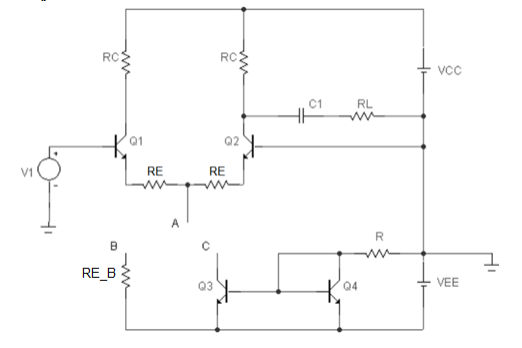
\includegraphics[height=90mm]{./imagenes/Circuito.png} }
		\caption{\small{\textit{ Circuito bajo estudio }}}
    \end{figure}
    Para esto utilizamos transisores BC548, de cuya hoja de datos se obtuvieron los siguientes valores:
    \begin{itemize}
        \item $h_{FE} = 300$
        \item $V_{BE} = \mV{0.7}$
        \item $V_A = \mV{-100}$
    \end{itemize}

\newpage
\section{Utilizando Fuente Espejo}
Al utilizar la fuente espejo para la polarización, el circuito quedaría de la siguiente manera:
\begin{figure}[H]
    \setlength{\abovecaptionskip}{0pt}
    \centering
    \captionsetup{labelformat=empty}
    \fbox{ 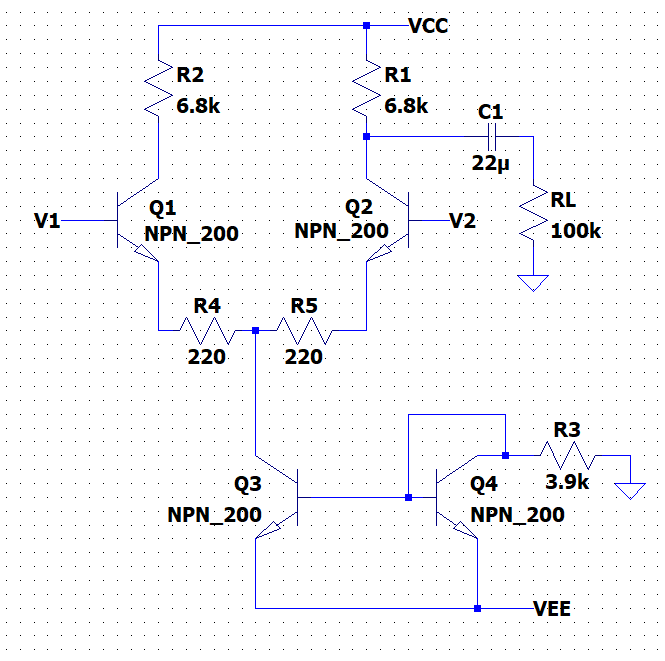
\includegraphics[width=130mm]{./imagenes/Circuito_Fuente.png} }
    \caption{\small{\textit{ Circuito }}}
\end{figure}
\newpage
\subsection{Estatico}
    Analisando el cirucito estático, se obtiene el siguiente circuito:
    \begin{figure}[H]
        \setlength{\abovecaptionskip}{0pt}
		\centering
		\captionsetup{labelformat=empty}
		\fbox{ 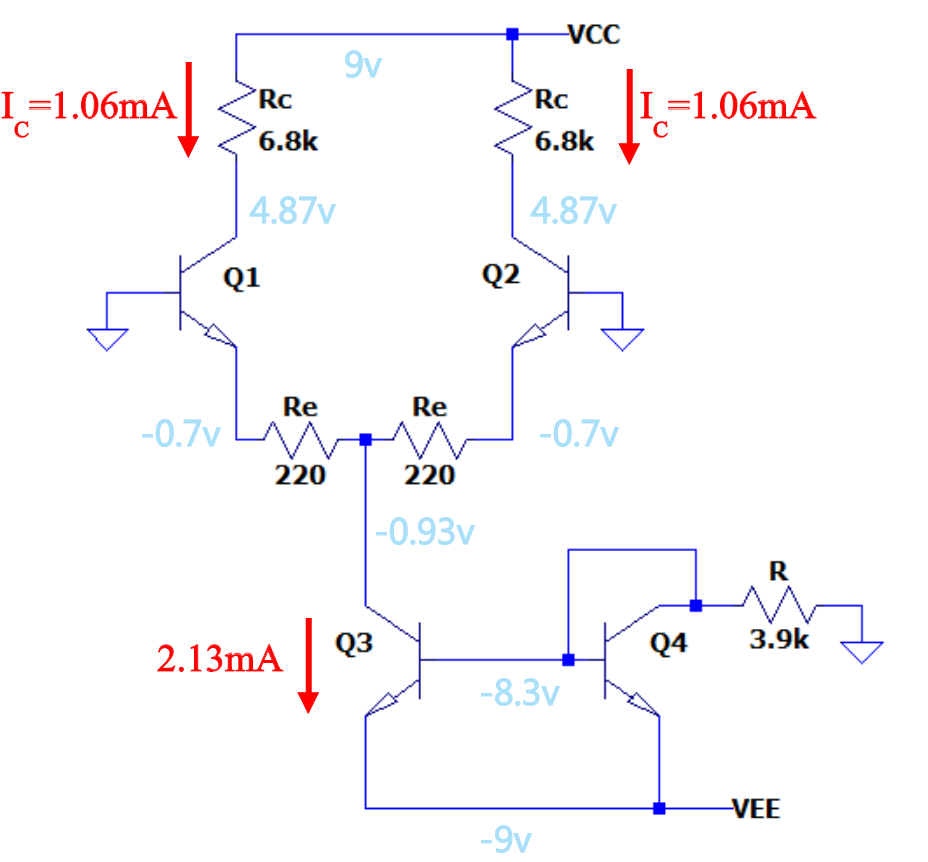
\includegraphics[width=140mm]{./imagenes/Circuito_Fuente_Estatico.png} }
		\caption{\small{\textit{ Circuito estático }}}
    \end{figure}


\subsection{Dinamico}
    Segun el punto Q calculado en el estatico:
    \begin{gather*}
        g_m = \SI{40}{\cfrac{1}{\volt}} \cdot I_C = \SI{40}{\cfrac{1}{\volt}} \cdot \mI{1.06} = \SI{42.4}{\cfrac{mA}{V}}
        \\ \\
        h_{ie} = \cfrac{h_{FE}}{g_m} = \cfrac{300}{\SI{42.4}{\cfrac{mA}{V}}} = \mR{7.07}
        \\ \\
        r_o = \cfrac{| V_A |}{I_C} = \cfrac{|\mV{-100}|}{\mI{1.06}} = \mR{94}
    \end{gather*}

    \newpage
    Analisando el cirucito dinámico en modo diferencial, se obtiene el siguiente circuito:
    \begin{figure}[H]
        \setlength{\abovecaptionskip}{0pt}
		\centering
		\captionsetup{labelformat=empty}
		\fbox{ 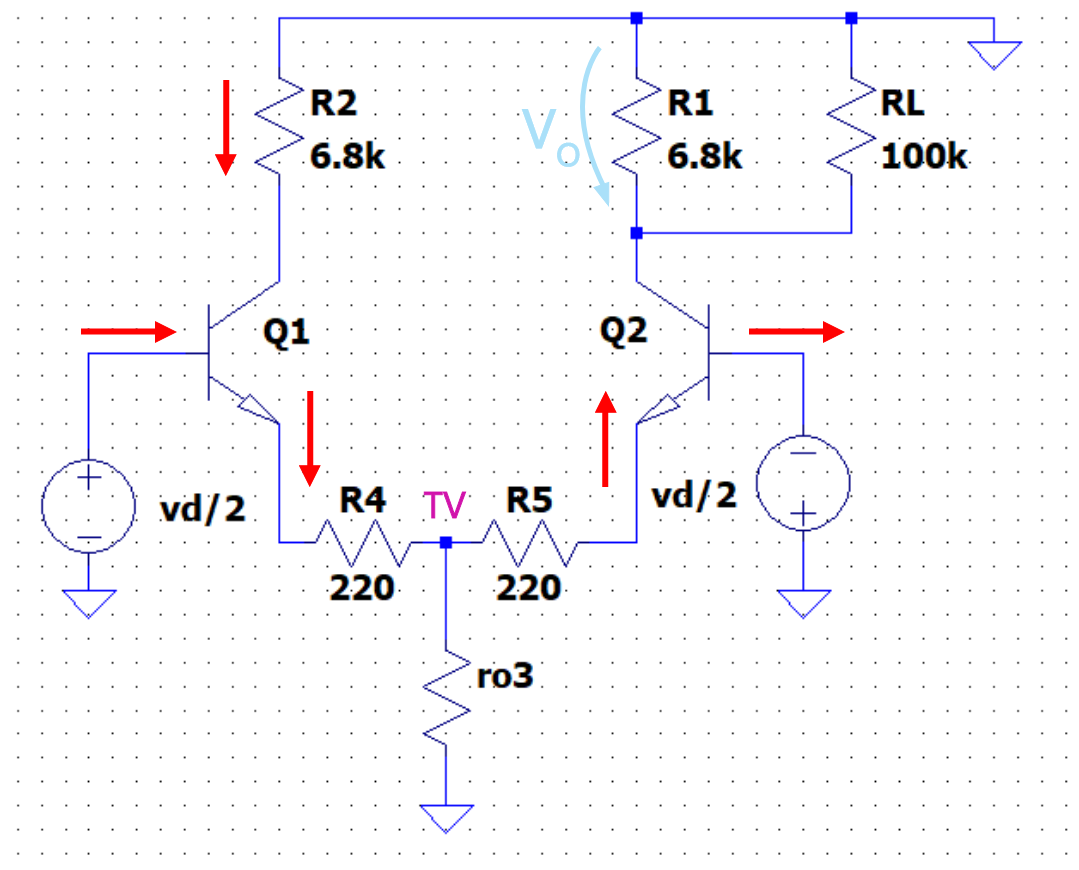
\includegraphics[width=130mm]{./imagenes/Circuito_Fuente_DinamicoDif.png} }
		\caption{\small{\textit{ Circuito dinámico }}}
    \end{figure}

    Y con estos valores podemos sacar las resistencias de entrada $R_i$ y de salida $R_o$ como:
    \begin{gather*}
        R_i = 2 ( h_{ie} + h_{FE} R_E ) = 2 ( \mR{7.07} + 300 \mR{0.22} ) = \mR{146}
        \\ \\
        R_o = \bigg( r_o \bigg( 1 + \cfrac{h_{FE} R_E}{R_{BT} + h_{ie} + R_E} \bigg) \bigg) \bigg/\bigg/ R_C\\
        R_o = \bigg( \mR{94} \cdot \bigg( 1 + \cfrac{300 \cdot \mR{0.22}}{\mR{7.07} + \mR{0.22}} \bigg) \bigg) \bigg/\bigg/ \mR{6.6}\\
        R_o = \parallelTwo{\mR{940}}{\mR{6.6}} = \mR{6.5}
    \end{gather*}

    Y segun el circuito dinamico en modo diferencial podemos plantear la ganancia en modo diferencial como:
    \begin{gather*}
        A_{vd} = \cfrac{v_o}{v_d} = \cfrac{g_m (\parallelTwo{R_C}{R_L})}{2 (1 + R_E g_m)}
            = \cfrac{ \SI{42.4}{\cfrac{mA}{V}} (\parallelTwo{6.8}{100}) }{ 2 (1 + \SI{42.4}{\cfrac{mA}{V}} \cdot \mR{0.22}) }
            = \cfrac{269.96}{20.66} = 13.07
    \end{gather*}
    \newpage
    A partir del circuito dinámico podemos plantear la ganancia en modo comun como:
    \begin{gather*}
        A_{vc} = \cfrac{g_m (\parallelTwo{R_C}{R_L})}{1 + g_m r_{o3} }
            = \cfrac{ \SI{42.4}{\cfrac{mA}{V}} (\parallelTwo{6.8}{100}) }{ 1 + \SI{42.4}{\cfrac{mA}{V}} \cdot \mR{47} }
            = \cfrac{269.96}{1991} = 0.13
    \end{gather*}

    Y podemos hallar la relacion de rechazo en modo común como:
    \begin{gather*}
        CMRR = \cfrac{A_{vd}}{A_{vc}} = \cfrac{13.07}{0.13} = 100.5
    \end{gather*}

\newpage
\section{Utilizando Resistencia}
Al utilizar una resistencia para la polarización, el circuito quedaría de la siguiente manera:
\begin{figure}[H]
    \setlength{\abovecaptionskip}{0pt}
    \centering
    \captionsetup{labelformat=empty}
    \fbox{ 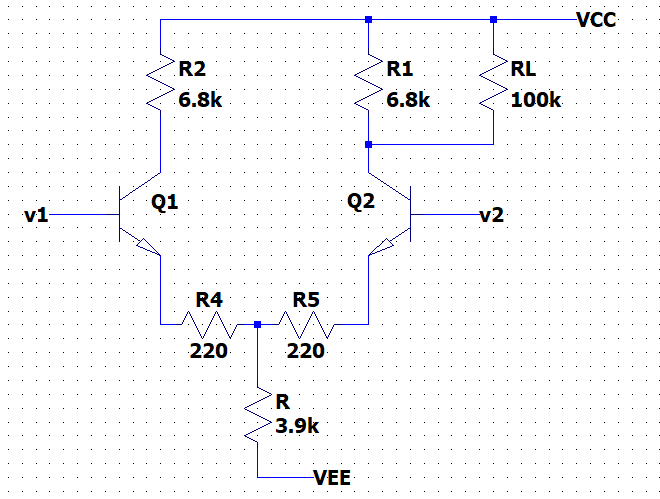
\includegraphics[height=90mm]{./imagenes/Circuito_Resistencia.png} }
    \caption{\small{\textit{ Circuito }}}
\end{figure}

    Donde $R = \mR{3.9}$ se determino de manera que se mantuviera constante la corriente $I_C$, manteniendose así también
    el circuito estático previamente analisado.
    \\
    De esta manera lo unico que cambiará en este caso será la ganancia en modo común la cual se calculará como:
        \begin{gather*}
            A_{vc} = \cfrac{g_m (\parallelTwo{R_C}{R_L})}{1 + g_m R }
                = \cfrac{ \SI{42.4}{\cfrac{mA}{V}} (\parallelTwo{6.8}{100}) }{ 1 + \SI{42.4}{\cfrac{mA}{V}} \cdot \mR{3.9} }
                = \cfrac{269.96}{166} = 1.62
        \end{gather*}
    
        Y podemos hallar la relacion de rechazo en modo común como:
        \begin{gather*}
            CMRR = \cfrac{A_{vd}}{A_{vc}} = \cfrac{13.07}{1.62} = 8.03
        \end{gather*}

\newpage
\section{Simulacion}
    \begin{figure}[H]
        \setlength{\abovecaptionskip}{0pt}
		\centering
		\captionsetup{labelformat=empty}
		\fbox{ 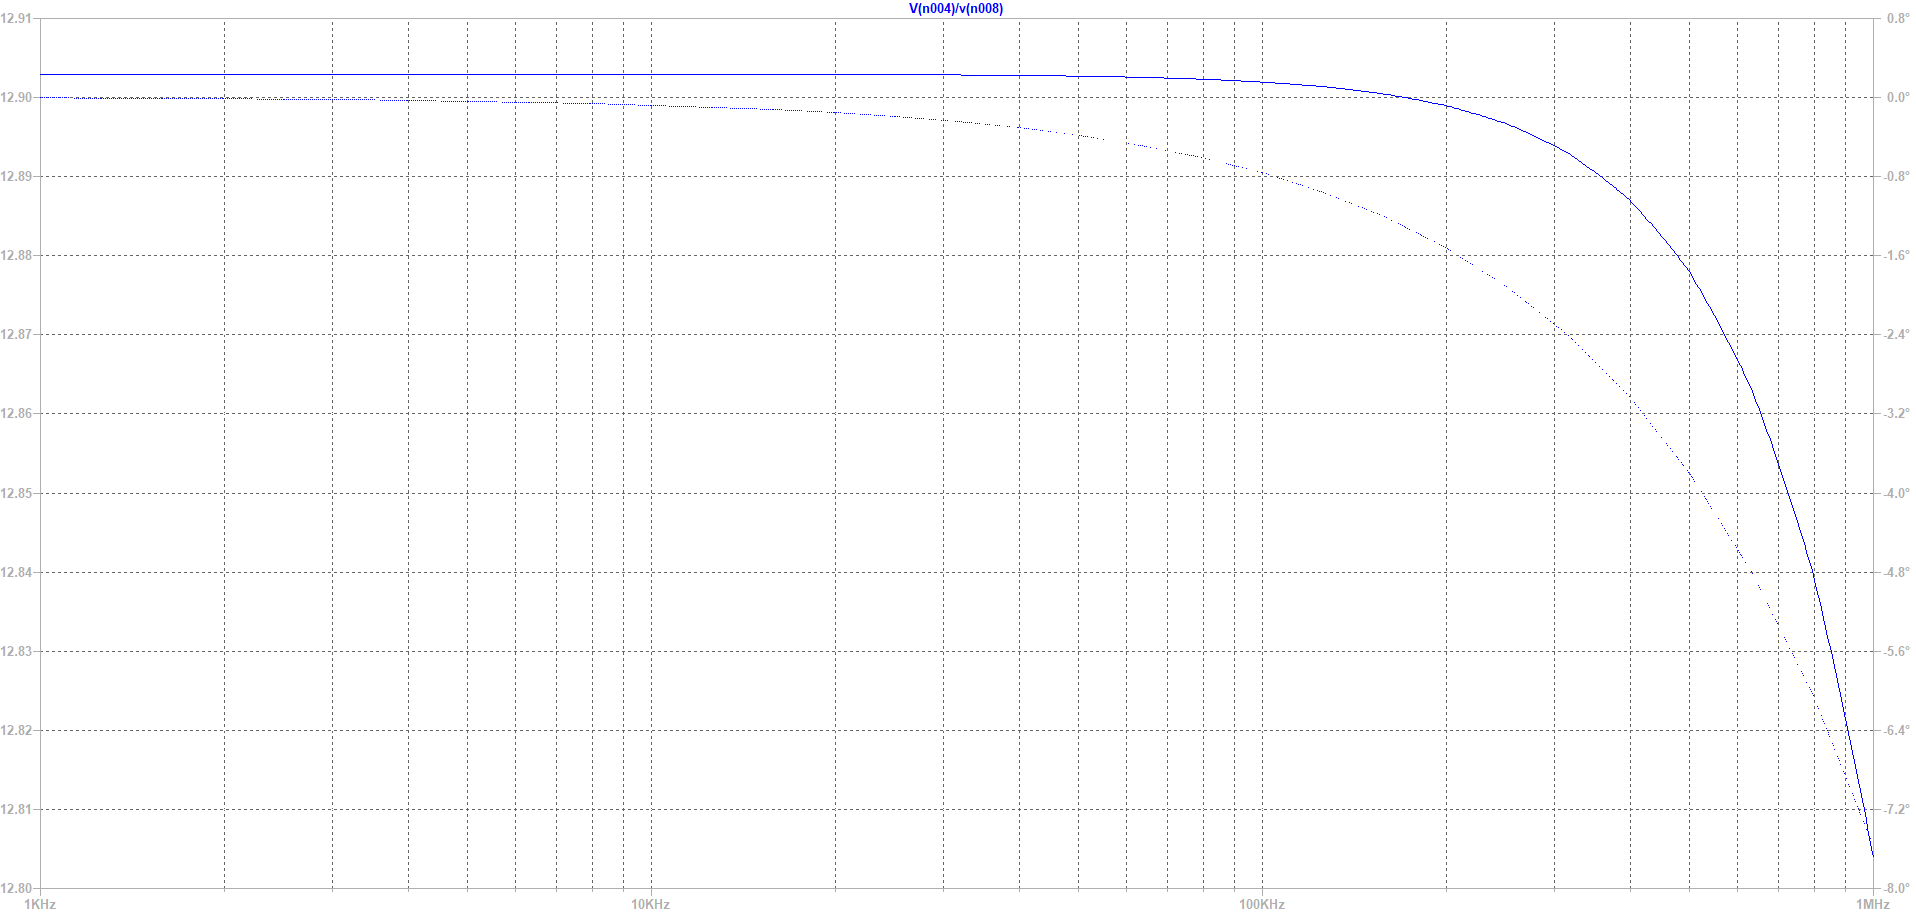
\includegraphics[height=80mm]{./imagenes/Curva_Ganancia.png} }
		\caption{\small{\textit{ Curva de ganancia en Modo Diferencial }}}
    \end{figure}
    El resto de los resultados se indican en la tabla presente en la siguiente seccion.


\newpage
\section{Cuadro de Resultados}
\begin{table}[h]
    \centering
    \begin{tabular}{|c|c|c|c|c|c|c|}
        \hline
                        &   \multicolumn{3}{|c|}{CON FUENTE}     &    \multicolumn{3}{|c|}{CON RESISTENCIA}   \\ \cline{2-7}
                        & CALCULADO & SIMULADO & MEDIDO          & CALCULADO & SIMULADO & MEDIDO  \\ \hline
        $V_{CE1}$       & 2.9 v     & 1.98 v   & 2.01 v          & 2.9 v     & 2.61 v   & 2.58 v  \\
        $V_{CE2}$       & 2.9 v     & 1.98 v   & 2.01 v          & 2.9 v     & 2.61 v   & 2.54 v  \\
        $V_{CE3}$       & 8.07 v    & 8.11 v   & 8.13 v          &  -        &  -       &  -      \\
        $V_{CE4}$       & 0.7 v     & 0.68 v   & 0.62 v          &  -        &  -       &  -      \\
        $I_{C1}$        & 1.06 mA   & 1.13 mA  & 1.02 mA         & 1.03 mA   & 1.03 mA  & 1.06 mA \\
        $I_{C2}$        & 1.06 mA   & 1.13 mA  & 1.02 mA         & 1.03 mA   & 1.03 mA  & 1.06 mA \\
        $I_{C3}$        & 2.13 mA   & 2.27 mA  & 2.03 mA         &  -        &  -       &  -      \\
        $I_{C4}$        & 2.13 mA   & 2.11 mA  & 2.04 mA         &  -        &  -       &  -      \\
        $Avd$           & 13.07     & 12.9     & 10.27           & 13.07     & 12.43    & 8.91    \\
        $Avc$           & 0.13      & 0.12     & 0.2             & 1.62      & 1.58     & 0.64    \\
        $CMRR$          & 100.5     & 107.5    & 51.3            & 8         & 7.87     & 13.9    \\
        $Ri$            & $\mR{146}$ & $\mR{139}$ & $\mR{126}$       & $\mR{146}$ & $\mR{137}$ & $\mR{112}$  \\
        $Ro$            & $\mR{6.6}$ & $\mR{6.2}$ & $\mR{5.6}$       & $\mR{6.6}$ & $\mR{6.2}$ & $\mR{5.6}$  \\ \hline
    \end{tabular}
\end{table}


\section{Conclusiones}
    Al realizar el circuito con componentes discretos notamos que para aquellas aplicaciones que requieran transistores "iguales",
    tal es el caso de la fuente compuesta por $Q_3$ y $Q_4$ y del diferencial compuesto por $Q_1$ y $Q_2$, se torna casi imposible el armado
    del mismo.

\end{document}
